% Coordenadas sobre la esfera y trigonometría esférica
% Números y figuras PNG: apunte/scripts/cap15_trigonometria_esferica.py (uv run python apunte/scripts/cap15_trigonometria_esferica.py)
\chapter{Coordenadas sobre la esfera y trigonometría esférica}\label{cap:esfera}

\section{La idea}

El capítulo~\ref{cap:elipsoide} dejó la esfera de radio \(\sqrt{MN}\) como reemplazo local del
elipsoide; ahora resolvemos triángulos sobre ella. Una poligonal corta se calcula en el plano:
los ángulos de un triángulo suman \(180^\circ\) y el error de cierre angular es error de
medición. Cuando los vértices se separan decenas o
cientos de kilómetros, esa cuenta deja de cerrar aunque las mediciones sean perfectas: la
superficie sobre la que se trazan los lados es curva. El modelo curvo más simple es la
esfera, y sobre ella hay fórmulas cerradas para todo lo que en el plano resuelve la
trigonometría elemental. Las deducimos con producto interno, producto vectorial,
determinante y rotaciones.

\paragraph{Convenciones del capítulo.} Esfera de centro \(o\) y radio \(R\) (casi todo en la
unitaria; al final se multiplica por \(R\)); cada punto se identifica con su vector unitario;
vértices \(A,B,C\) con vectores \(u,v,w\), lados opuestos \(a,b,c\), que son \emph{ángulos}, y
ángulos del triángulo también \(A,B,C\) (el contexto decide); latitud \(\varphi\) positiva al
norte, longitud \(\lambda\) positiva al este y acimut \(\alpha\) desde el norte en sentido
horario (sección~\ref{sec:acimut-campo}).

\subsection{Coordenadas sobre la esfera}

El punto de latitud \(\varphi\) y longitud \(\lambda\) de la esfera unitaria es
\[
  \hat r(\varphi,\lambda)=
  \begin{pmatrix}\cos\varphi\cos\lambda\\ \cos\varphi\sin\lambda\\ \sin\varphi\end{pmatrix},
\]
con el eje \(z\) hacia el polo norte y el eje \(x\) en el meridiano de longitud cero. Al
mover un poco la longitud, el punto se desplaza hacia el este; al mover la latitud, hacia el
norte. Derivando,
\[
  \frac{\partial\hat r}{\partial\lambda}=\cos\varphi\,\hat e,\qquad
  \frac{\partial\hat r}{\partial\varphi}=\hat n,\qquad
  \hat e=\begin{pmatrix}-\sin\lambda\\ \cos\lambda\\ 0\end{pmatrix},\quad
  \hat n=\begin{pmatrix}-\sin\varphi\cos\lambda\\ -\sin\varphi\sin\lambda\\ \cos\varphi\end{pmatrix}.
\]
Los tres vectores \(\hat e,\hat n,\hat r\) son unitarios y perpendiculares entre sí, y en ese
orden forman una base de orientación positiva: \(\hat e\times\hat n=\hat r\). Es la base
local \emph{este, norte, vertical} de cada punto. El factor \(\cos\varphi\) de la primera
derivada dice que un grado de longitud mide menos cuanto más cerca del polo: los meridianos
convergen. Esa convergencia es la que hace cambiar el acimut a lo largo de un camino recto
sobre la esfera.

\paragraph{El orden de los giros.} Sobre una esfera, los giros alrededor de ejes distintos
juegan el papel de los centros distintos del plano (sección~\ref{sec:componer-centros}): un
vaso girado un cuarto de vuelta alrededor de un eje vertical y después de uno horizontal no
queda como en el orden inverso. Lo mismo pasa al ubicar un punto con longitud y latitud.

\begin{idea}[Sobre la esfera, todo se mide con ángulos]
Con producto interno se miden los lados; con producto vectorial, los ángulos. El radio \(R\)
aparece una sola vez, al pasar de radianes a metros.
\end{idea}

\subsection{Círculos máximos y triángulos esféricos}

\begin{definicion}[Círculo máximo]
Un \emph{círculo máximo} es la intersección de la esfera con un plano que pasa por el
centro. Si \(k\) es un vector unitario normal al plano, el círculo máximo es
\(\{x:\ \|x\|=1,\ k\cdot x=0\}\). Por dos puntos \(u,v\) no opuestos pasa uno solo: el del
plano de normal \(k=u\times v/\|u\times v\|\).
\end{definicion}

El ecuador y los meridianos son círculos máximos; los paralelos distintos del ecuador no lo
son, porque su plano no pasa por el centro. El arco menor de círculo máximo entre dos puntos
es el camino más corto entre ellos sobre la esfera, la geodésica de la esfera; ese hecho lo
aceptamos sin demostración. Lo que sí se usa es la medida del arco: entre \(u\) y \(v\) el arco mide el ángulo \(\theta\) con
\(\cos\theta=u\cdot v\), en radianes sobre la esfera unitaria y \(R\theta\) sobre la de radio
\(R\).

\begin{definicion}[Triángulo esférico]
Sean \(u,v,w\) tres vectores unitarios linealmente independientes, los vértices \(A,B,C\).
El \emph{triángulo esférico} \(ABC\) es la región de la esfera limitada por los tres arcos
menores de círculo máximo que los unen. Sus \emph{lados} son los ángulos al centro
\[
  \cos a=v\cdot w,\qquad \cos b=u\cdot w,\qquad \cos c=u\cdot v,
\]
con \(0<a,b,c<\pi\). Su \emph{ángulo} en \(A\) es el ángulo diedro entre los planos \(OAB\) y
\(OAC\), igual al ángulo entre las tangentes en \(A\) a los dos lados que salen de ese
vértice.
\end{definicion}

\begin{figure}[htbp]
\centering
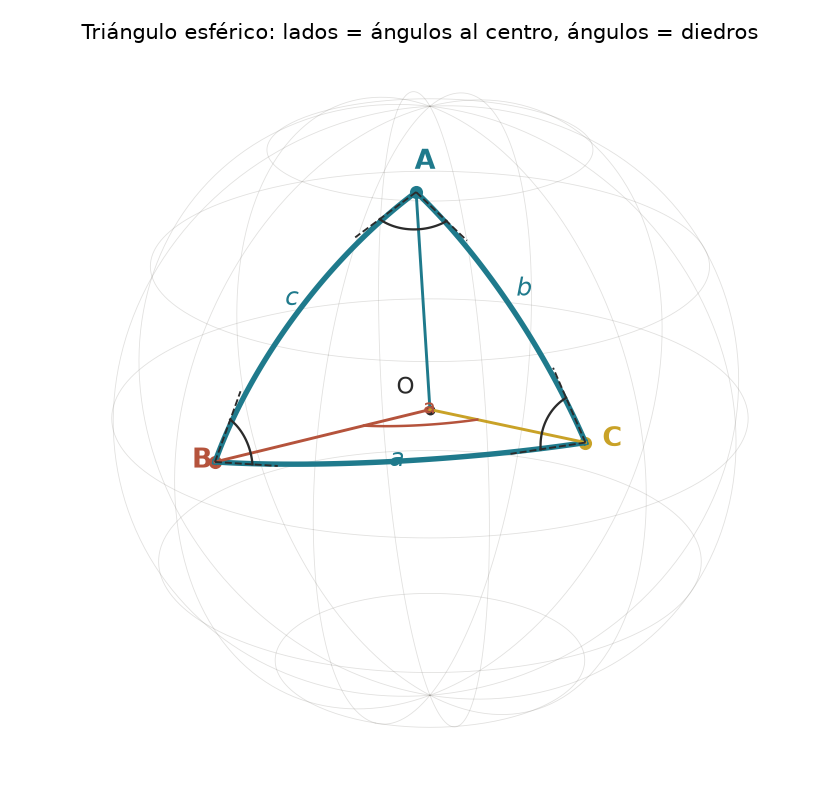
\includegraphics[width=.62\linewidth]{figuras/esfera/esfera_triangulo.png}
\caption{Triángulo esférico de vértices \(A,B,C\). El lado \(a\) es el ángulo al centro
entre los vectores de \(B\) y de \(C\) (arco chico en rust junto a \(o\)); los ángulos del
triángulo son los que forman, en cada vértice, las tangentes a los dos lados (trazos
negros). Generada con \texttt{apunte/scripts/cap15\_trigonometria\_esferica.py}.}
\label{fig:esfera-triangulo}
\end{figure}

La figura~\ref{fig:esfera-triangulo} muestra los dos tipos de elementos. Los lados no se
miden en metros: son ángulos. Los ángulos del triángulo tampoco se ven en el centro: viven en
el plano tangente de cada vértice. La tangente en \(A\) al lado \(AB\) es la parte de \(v\)
perpendicular a \(u\), \(v-(u\cdot v)\,u\), y lo mismo con \(w\). Girando esas dos tangentes
un cuarto de vuelta alrededor de \(u\) se obtienen \(u\times v\) y \(u\times w\), las normales
de los planos \(OAB\) y \(OAC\); por eso el ángulo entre tangentes y el ángulo entre normales
coinciden:
\[
  \cos A=\frac{(u\times v)\cdot(u\times w)}{\|u\times v\|\,\|u\times w\|}.
\]

\unidadInteractiva{14_trigonometria_esferica}{Trigonometría esférica}{Explorá: con el caso «a mano» mové la latitud y la longitud de \(C\) y mirá cómo crecen a la vez la suma de los ángulos y el área del triángulo.}

\begin{idea}[Un triángulo esférico son tres planos por el centro]
Toda la trigonometría esférica es geometría de tres vectores unitarios y de los planos que
generan de a dos.
\end{idea}

\subsection{Los ángulos suman más de \texorpdfstring{\(180^\circ\)}{180°}}

El ejemplo más simple ya muestra la diferencia con el plano.

\begin{ejemplo}[El octante]\label{ej:esfera-octante}
Sean \(u=(0,0,1)\) (el polo norte), \(v=(1,0,0)\) y \(w=(0,1,0)\) (dos puntos del ecuador a
\(90^\circ\) de longitud). Los tres productos internos son cero, de modo que
\(a=b=c=90^\circ\). Las normales \(u\times v=(0,1,0)\) y \(u\times w=(-1,0,0)\) son
perpendiculares, así que \(A=90^\circ\), y por simetría \(B=C=90^\circ\). Los ángulos suman
\(270^\circ\): sobran \(90^\circ=\pi/2\). El triángulo cubre un octavo de la esfera, de área
\(4\pi/8=\pi/2\) en la esfera unitaria: el sobrante coincide con el área. El
teorema~\ref{teo:girard} dice que no es casualidad.
\end{ejemplo}

\section{Construcciones, cuentas y ejemplos}

\subsection{Teorema del coseno}

\begin{teorema}[Teorema del coseno para los lados]\label{teo:coseno-lados}
En todo triángulo esférico
\[
  \cos a=\cos b\cos c+\sin b\sin c\cos A .
\]
\end{teorema}

\begin{demostracion}
Los lados y los ángulos se definen con productos internos, que no cambian al aplicar una
rotación (proposición~\ref{prop:propiedades-R} y sección~\ref{sec:rot-3d}); se puede elegir
entonces el sistema de coordenadas. Se pone \(A\) en el polo, \(u=(0,0,1)\), y \(B\) sobre el
meridiano de longitud cero a distancia angular \(c\) del polo, \(v=(\sin c,0,\cos c)\). El
punto \(C\) está a distancia \(b\) del polo, sobre el meridiano que forma con el anterior el
ángulo \(A\) (en el polo, el ángulo entre meridianos es la diferencia de longitudes):
\(w=(\sin b\cos A,\ \sin b\sin A,\ \cos b)\). Entonces
\[
  \cos a=v\cdot w=\sin c\sin b\cos A+\cos c\cos b . \qedhere
\]
\end{demostracion}

La misma cuenta sin coordenadas usa la identidad de Lagrange,
\((u\times v)\cdot(u\times w)=(u\cdot u)(v\cdot w)-(u\cdot w)(v\cdot u)\), que se verifica
desarrollando las componentes del producto vectorial (capítulo~\ref{cap:subespacios}). El
primer miembro es \(\|u\times v\|\,\|u\times w\|\cos A=\sin c\sin b\cos A\) y el segundo,
\(\cos a-\cos b\cos c\).

\paragraph{Una Tierra chica es plana.} Si los lados son chicos, \(\cos x\approx1-x^2/2\) y
\(\sin x\approx x\). Llevando esto al teorema y despreciando los términos de cuarto orden
queda \(a^2=b^2+c^2-2bc\cos A\): el teorema del coseno del plano. La trigonometría plana es
el límite de la esférica para triángulos chicos frente al radio.

\subsection{Teorema del seno}

\begin{teorema}[Teorema del seno]\label{teo:seno-esferico}
En todo triángulo esférico
\[
  \frac{\sin A}{\sin a}=\frac{\sin B}{\sin b}=\frac{\sin C}{\sin c}
  =\frac{|\det[u\ v\ w]|}{\sin a\sin b\sin c}.
\]
\end{teorema}

\begin{demostracion}
Para tres vectores cualesquiera vale \((u\times v)\times(u\times w)=\det[u\ v\ w]\,u\). En
efecto, la fórmula del doble producto vectorial,
\(x\times(y\times z)=(x\cdot z)\,y-(x\cdot y)\,z\), con \(x=u\times v\), da
\(\bigl((u\times v)\cdot w\bigr)u-\bigl((u\times v)\cdot u\bigr)w\); el segundo término es
cero y el primero es el producto mixto, igual a \(\det[u\ v\ w]\)
(sección~\ref{sec:producto-mixto}). Tomando normas, como \(\|u\|=1\),
\[
  |\det[u\ v\ w]|=\|u\times v\|\,\|u\times w\|\sin A=\sin c\sin b\sin A .
\]
El determinante no depende del vértice elegido (salvo el signo, que se pierde con el valor
absoluto), así que repitiendo la cuenta desde \(B\) y desde \(C\),
\(\sin c\sin b\sin A=\sin a\sin c\sin B=\sin a\sin b\sin C\). Dividiendo por
\(\sin a\sin b\sin c\) se obtiene el enunciado.
\end{demostracion}

El volumen \(|\det[u\ v\ w]|\) del paralelepípedo de los tres vértices aparece así como el
invariante del triángulo: el mismo número mirado desde cada vértice.

\subsection{El triángulo polar y el teorema del coseno para los ángulos}

\begin{definicion}[Triángulo polar]
Con los vértices ordenados de modo que \(\det[u\ v\ w]>0\), el \emph{triángulo polar} de
\(ABC\) tiene vértices
\[
  u'=\frac{v\times w}{\sin a},\qquad v'=\frac{w\times u}{\sin b},\qquad w'=\frac{u\times v}{\sin c}:
\]
cada vértice polar es el polo del lado opuesto, del lado en que está el vértice original.
\end{definicion}

\begin{proposicion}\label{prop:polar}
Los lados del triángulo polar son los suplementos de los ángulos del original, y sus ángulos
son los suplementos de los lados:
\(a'=\pi-A,\ b'=\pi-B,\ c'=\pi-C\) y \(A'=\pi-a,\ B'=\pi-b,\ C'=\pi-c\).
\end{proposicion}

\begin{demostracion}
El lado \(a'\) es el ángulo entre \(v'\) y \(w'\), o sea entre \(w\times u\) y
\(u\times v\). Como \(w\times u=-(u\times w)\), ese ángulo es el suplemento del ángulo entre
\(u\times v\) y \(u\times w\), que es \(A\). Lo mismo para \(b'\) y \(c'\). Para los ángulos,
la identidad de la demostración del teorema~\ref{teo:seno-esferico} da
\(v'\times w'\) paralelo a \((w\times u)\times(u\times v)=\det[w\ u\ v]\,u=\det[u\ v\ w]\,u\):
como \(\det[u\ v\ w]>0\), el polar del polar es el triángulo original. Aplicando la primera parte al triángulo polar,
\(a=\pi-A'\), que es \(A'=\pi-a\).
\end{demostracion}

\begin{teorema}[Teorema del coseno para los ángulos]\label{teo:coseno-angulos}
En todo triángulo esférico
\[
  \cos A=-\cos B\cos C+\sin B\sin C\cos a .
\]
\end{teorema}

\begin{demostracion}
Se aplica el teorema~\ref{teo:coseno-lados} al triángulo polar,
\(\cos a'=\cos b'\cos c'+\sin b'\sin c'\cos A'\), y se reemplaza con la
proposición~\ref{prop:polar}: \(-\cos A=\cos B\cos C-\sin B\sin C\cos a\).
\end{demostracion}

Esta fórmula no tiene análogo plano: en el plano los tres ángulos no determinan los lados (dos
triángulos semejantes tienen los mismos ángulos). En la esfera sí, y la razón es que la
esfera tiene una escala propia, su radio.

\begin{ejemplo}[Tres ciudades]\label{ej:esfera-tres-ciudades}
Sobre la esfera de radio \(R=6371\) km tomamos, con coordenadas geográficas aproximadas,
Buenos Aires \((-34{,}6^\circ;\ -58{,}4^\circ)\), Córdoba \((-31{,}4^\circ;\ -64{,}2^\circ)\) y
Mendoza \((-32{,}9^\circ;\ -68{,}8^\circ)\), vértices \(A\), \(B\) y \(C\). Con
\(\hat r(\varphi,\lambda)\), \(u\approx(0{,}4313;\ -0{,}7011;\ -0{,}5678)\),
\(v\approx(0{,}3715;\ -0{,}7685;\ -0{,}5210)\) y \(w\approx(0{,}3036;\ -0{,}7828;\ -0{,}5432)\).

\emph{Lados}, por producto interno: \(a\) (Córdoba--Mendoza) \(=4{,}1730^\circ\), o sea
\(464{,}02\) km; \(b\) (Buenos Aires--Mendoza) \(=8{,}8085^\circ=979{,}46\) km; \(c\) (Buenos
Aires--Córdoba) \(=5{,}8208^\circ=647{,}24\) km.

\emph{Ángulos}, por el ángulo entre normales: en Buenos Aires \(A=23{,}5351^\circ\), en
Córdoba \(B=122{,}8281^\circ\), en Mendoza \(C=33{,}8154^\circ\). Suman \(180{,}1785^\circ\).

\emph{Controles.} El teorema del coseno da \(\cos a=0{,}997349\) por los dos miembros; el del
coseno para los ángulos, \(\cos A=0{,}916816\) por los dos miembros; y los tres cocientes
\(\sin a/\sin A\), \(\sin b/\sin B\), \(\sin c/\sin C\) valen \(0{,}182235\).

El sobrante de \(0{,}1785^\circ=642{,}7''\) no es error de cuenta: es el exceso esférico de
la sección~\ref{sec:exceso-esferico}.
\end{ejemplo}

\subsection{Recorrer el triángulo es componer rotaciones}

Ir de \(A\) a \(B\) por el lado \(c\) es rotar: la rotación de eje
\(k_{AB}=u\times v/\|u\times v\|\), perpendicular al plano del círculo máximo, y ángulo \(c\)
lleva \(u\) a \(v\) y mueve cada punto del lado sobre el propio lado
(capítulo~\ref{cap:rotaciones}; su matriz es la de Rodrigues, apéndice~\ref{ap:rot3d}).
Llamamos \(R_{AB}\), \(R_{BC}\) y \(R_{CA}\) a las tres rotaciones a lo largo de los lados. La composición \(R_{CA}R_{BC}R_{AB}\) lleva \(u\) a \(v\),
\(v\) a \(w\) y \(w\) de vuelta a \(u\): deja fijo \(A\), así que es una rotación de eje \(u\)
(teorema~\ref{teo:euler-eje}). La pregunta es cuánto gira.

\begin{proposicion}[El giro de la vuelta es el exceso]\label{prop:vuelta-exceso}
Si el triángulo \(ABC\) se recorre en sentido antihorario visto desde afuera
(\(\det[u\ v\ w]>0\)), la composición \(R_{CA}R_{BC}R_{AB}\) es la rotación de eje \(u\) y
ángulo \(A+B+C-\pi\).
\end{proposicion}

\begin{demostracion}
Basta seguir un vector tangente en \(A\). Cada rotación \(R_{XY}\) lleva el plano tangente en
\(X\) al plano tangente en \(Y\), conserva los ángulos y la orientación, y lleva la tangente
al lado \(XY\) en \(X\) (apuntando hacia \(Y\)) a la tangente al mismo lado en \(Y\) (apuntando
hacia adelante, más allá de \(Y\)). Sea \(t\) la tangente en \(A\) hacia \(B\). Después de
\(R_{AB}\), \(t\) es la continuación del lado \(AB\) en \(B\). La tangente hacia \(C\) se
obtiene de esa continuación girando el ángulo exterior \(\pi-B\) en sentido antihorario; o
sea, \(t\) es la tangente hacia \(C\) girada \(-(\pi-B)\). La rotación \(R_{BC}\) conserva esa
relación, y en \(C\) el mismo argumento suma el ángulo exterior \(\pi-C\): \(t\) queda como la
tangente hacia \(A\) girada \(-(\pi-B)-(\pi-C)\). Después de \(R_{CA}\), en \(A\), la tangente
hacia \(B\) es la continuación del lado \(CA\) girada \(\pi-A\). En total, la imagen de \(t\)
es \(t\) girada
\[
  -(\pi-A)-(\pi-B)-(\pi-C)=A+B+C-3\pi\equiv A+B+C-\pi\pmod{2\pi}. \qedhere
\]
\end{demostracion}

La cuenta numérica con el triángulo del ejemplo~\ref{ej:esfera-tres-ciudades}, donde
\(\det[u\ v\ w]\approx6{,}20\cdot10^{-3}>0\), confirma el enunciado: la composición de las
tres matrices de Rodrigues tiene eje \(u\) (el producto interno del eje con \(u\) es
\(1{,}000000000\)) y ángulo \(3{,}1159457\cdot10^{-3}\) rad, que coincide con
\(A+B+C-\pi\) hasta \(6\cdot10^{-14}\). En el plano la misma vuelta no gira nada: las tres
traslaciones a lo largo de los lados componen la identidad. El giro residual es la huella de
la curvatura.

\subsection{Exceso esférico y teorema de Girard}\label{sec:exceso-esferico}

\begin{definicion}[Exceso esférico]
El \emph{exceso esférico} de un triángulo esférico es
\(\varepsilon=A+B+C-\pi\).
\end{definicion}

Para calcular áreas se usan los \emph{husos} (o lúnulas): la región entre dos semicírculos
máximos que unen dos puntos opuestos. Un huso de ángulo \(\alpha\) tiene área \(2\alpha R^2\).
En efecto, las rotaciones alrededor del eje que une sus dos puntas conservan el área y llevan
un huso a otro del mismo ángulo; el área de un huso es entonces proporcional a su ángulo, y
como el huso de ángulo \(2\pi\) es la esfera entera, de área \(4\pi R^2\), la constante es
\(2R^2\).

\begin{teorema}[Girard]\label{teo:girard}
El área de un triángulo esférico sobre la esfera de radio \(R\) es
\[
  S=R^2\,\varepsilon=R^2(A+B+C-\pi).
\]
\end{teorema}

\begin{demostracion}
Los tres círculos máximos que contienen los lados cortan la esfera en ocho triángulos: \(ABC\),
su antípoda \(A^*B^*C^*\) (el de los vértices opuestos), de la misma área \(S\), y otros seis.
Por el vértice \(A\) pasan dos de esos círculos; limitan un huso de ángulo \(A\) que contiene a
\(ABC\), y el huso opuesto, de ángulo \(A\), que contiene a \(A^*B^*C^*\). Lo mismo en \(B\) y
en \(C\): seis husos en total (figura~\ref{fig:esfera-lunulas}), cuyas áreas suman
\[
  2\,(2AR^2+2BR^2+2CR^2)=4R^2(A+B+C).
\]
Esos seis husos cubren la esfera: cada punto que no está en \(ABC\) ni en su antípoda cae en
exactamente uno de ellos, mientras que \(ABC\) está en los tres husos de sus vértices y
\(A^*B^*C^*\) en los tres opuestos. La suma cuenta la esfera una vez y cada uno de esos dos
triángulos dos veces de más:
\[
  4R^2(A+B+C)=4\pi R^2+2S+2S .
\]
Despejando, \(S=R^2(A+B+C-\pi)\).
\end{demostracion}

\begin{figure}[htbp]
\centering
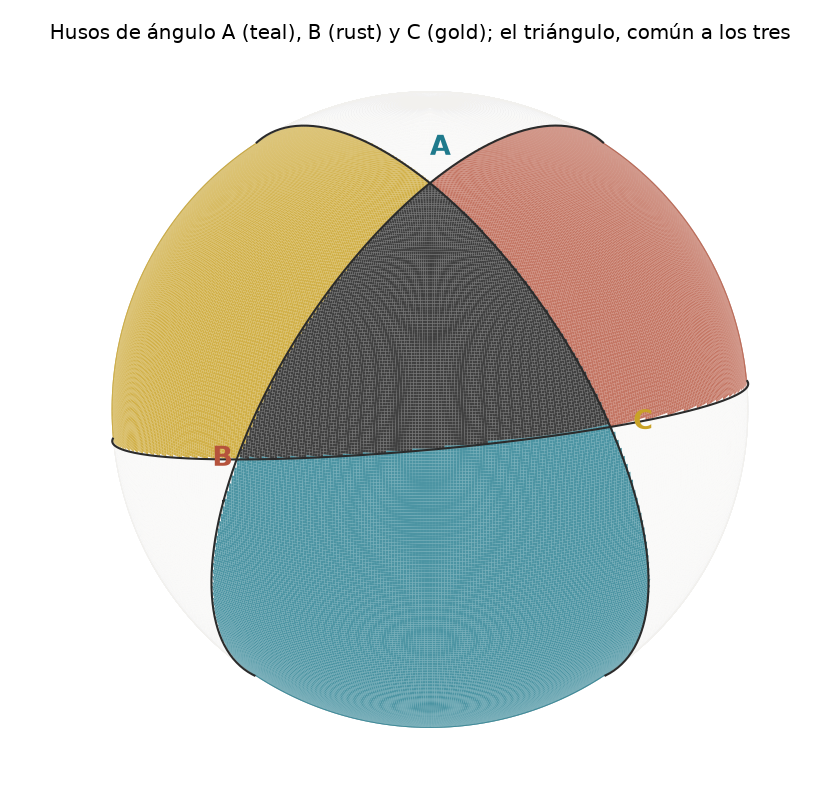
\includegraphics[width=.58\linewidth]{figuras/esfera/esfera_lunulas.png}
\caption{Los husos de Girard: de ángulo \(A\) (teal), \(B\) (rust) y \(C\) (gold). Los tres se
superponen solo en el triángulo \(ABC\) (oscuro); en la cara oculta están los tres husos
opuestos, que se superponen en el triángulo antípoda. Generada con
\texttt{apunte/scripts/cap15\_trigonometria\_esferica.py}.}
\label{fig:esfera-lunulas}
\end{figure}

El octante del ejemplo~\ref{ej:esfera-octante} cumple el teorema:
\(\varepsilon=\pi/2\), un octavo de \(4\pi\). Un polígono esférico de \(n\) lados se divide en
\(n-2\) triángulos desde un vértice, y sumando queda \(S=R^2\bigl(\sum\text{ángulos}-(n-2)\pi\bigr)\).

\begin{ejemplo}[Exceso y área del triángulo de las tres ciudades]\label{ej:esfera-exceso-ciudades}
Para el triángulo del ejemplo~\ref{ej:esfera-tres-ciudades}, \(\varepsilon=0{,}1785^\circ
=642{,}7''=3{,}1159\cdot10^{-3}\) rad, y el área es
\(\varepsilon R^2=3{,}1159\cdot10^{-3}\cdot6371^2\approx126\,475\) km\(^2\). Dos controles
independientes de la suma de ángulos dan el mismo \(\varepsilon\) hasta \(4\cdot10^{-17}\)
rad: la fórmula de L'Huilier,
\[
  \tan\frac\varepsilon4=\sqrt{\tan\frac s2\,\tan\frac{s-a}2\,\tan\frac{s-b}2\,\tan\frac{s-c}2},
  \qquad s=\frac{a+b+c}2,
\]
que da el exceso a partir de los lados (es el análogo esférico de la fórmula de Herón; se
deduce del teorema del coseno con identidades trigonométricas, y aquí no se la demuestra), y
la fórmula del determinante,
\(\tan(\varepsilon/2)=|\det[u\ v\ w]|/(1+u\cdot v+v\cdot w+w\cdot u)\), que lo da a partir de
los vértices (también sin demostración). En una poligonal entre estas tres ciudades,
\(10'43''\) de la suma angular son geometría de la esfera y no error de medición.
\end{ejemplo}

\subsection{Simulaciones}

\unidadInteractiva{14_trigonometria_esferica}{Trigonometría esférica}{Verificá: elegí el caso «octante» y comprobá que la suma da \(270^\circ\) y el exceso un octavo de \(4\pi\); después elegí «triángulo chico» y comprobá que la suma queda a centésimas de grado de \(180^\circ\).}

\section{En profundidad}

\subsection{Triángulos chicos: exceso y teorema de Legendre}

En geodesia los triángulos tienen lados de decenas de kilómetros sobre un radio de unos
\(6370\) km. Para ellos hay dos aproximaciones que evitan la trigonometría esférica completa.

\paragraph{El exceso por el área plana.} Si \(S\) es el área del triángulo plano con los
mismos lados (por Herón, o \(\frac12 bc\sin A\)), el teorema de Girard con \(S\) en lugar del
área esférica da \(\varepsilon\approx S/R^2\). La diferencia entre el área plana y la esférica es relativa al cuadrado de los lados medidos
en radianes, de modo que el error de la aproximación es mucho menor que \(\varepsilon\) mismo.
Un triángulo equilátero de \(40\) km de lado tiene \(\varepsilon\approx3{,}5''\) sobre la
Tierra (ejercicio~\ref{ex:esfera-legendre}); uno de \(1\) km, de área \(0{,}433\) km\(^2\), apenas \(0{,}0022''\).

\begin{teorema}[Legendre]\label{teo:legendre}
Si los lados de un triángulo esférico son chicos frente a \(R\), el triángulo plano con los
mismos lados (medidos en longitud, \(Ra\), \(Rb\), \(Rc\)) tiene por ángulos
\[
  A-\frac\varepsilon3,\qquad B-\frac\varepsilon3,\qquad C-\frac\varepsilon3,
\]
La corrección \(\varepsilon/3\) es de segundo orden en los lados medidos en radianes (porque
\(\varepsilon\approx S/R^2\)), y el error que queda después de aplicarla es de cuarto orden.
\end{teorema}

Lo enunciamos sin demostración (la prueba desarrolla el teorema del coseno esférico en serie
de potencias de los lados hasta cuarto orden y compara con el plano). Lo que se usa es la
consecuencia práctica: \emph{se resuelve el
triángulo como plano después de restar a cada ángulo un tercio del exceso}. Para el
triángulo grande del ejemplo~\ref{ej:esfera-tres-ciudades} el ángulo plano en Buenos Aires,
con los mismos lados, es \(23{,}475527^\circ\), y el esférico menos un tercio del exceso es
\(23{,}475550^\circ\): aun con lados de casi \(1000\) km la diferencia es \(0{,}08''\).

\subsection{Problema directo e inverso sobre la esfera}\label{sec:problema-directo-inverso}

Los dos problemas básicos de la geodesia son el \emph{directo}, que desde un punto
\(P_1=(\varphi_1,\lambda_1)\), con acimut de partida \(\alpha_1\) y distancia angular
\(\sigma\), busca el punto de llegada \(P_2=(\varphi_2,\lambda_2)\) y el acimut de llegada
\(\alpha_2\), y el \emph{inverso}, que dados \(P_1\) y \(P_2\) busca la distancia \(\sigma\) y
los acimutes \(\alpha_1\) y \(\alpha_2\). El acimut de llegada \(\alpha_2\) es la dirección en que se sigue avanzando al llegar a
\(P_2\); el contraacimut, la dirección en que se ve \(P_1\) desde \(P_2\), es
\(\alpha_2\pm180^\circ\).

\paragraph{El triángulo polo--punto--punto.} Los dos puntos y el polo norte \(N\) forman un
triángulo esférico con lados \(90^\circ-\varphi_1\) (de \(N\) a \(P_1\)),
\(90^\circ-\varphi_2\) (de \(N\) a \(P_2\)) y \(\sigma\); su ángulo en \(N\) es
\(\Delta\lambda=\lambda_2-\lambda_1\), su ángulo en \(P_1\) es el acimut \(\alpha_1\) y su
ángulo en \(P_2\) es \(180^\circ-\alpha_2\) (cuando \(P_2\) está al este de \(P_1\) y los
ángulos están entre \(0\) y \(\pi\); las fórmulas vectoriales de abajo valen en todos los casos).
El teorema del coseno en el vértice \(N\) da la distancia:
\[
  \cos\sigma=\sin\varphi_1\sin\varphi_2+\cos\varphi_1\cos\varphi_2\cos\Delta\lambda .
\]

\paragraph{Inverso, por vectores.} En \(P_1\), la tangente hacia \(P_2\) es la parte de
\(\hat r_2\) perpendicular a \(\hat r_1\): \(\hat r_2-\cos\sigma\,\hat r_1=\sin\sigma\,t\), con
\(t\) unitario. Su acimut es el ángulo de \(t\) medido desde \(\hat n_1\) hacia \(\hat e_1\),
y como \(\hat e_1\) y \(\hat n_1\) son perpendiculares a \(\hat r_1\), sus componentes son
\(\hat r_2\cdot\hat e_1\) y \(\hat r_2\cdot\hat n_1\). Con las fórmulas de \(\hat r\),
\(\hat e\) y \(\hat n\):
\[
  \hat r_2\cdot\hat e_1=\cos\varphi_2\sin\Delta\lambda,\qquad
  \hat r_2\cdot\hat n_1=\cos\varphi_1\sin\varphi_2-\sin\varphi_1\cos\varphi_2\cos\Delta\lambda,
\]
\[
  \boxed{\ \alpha_1=\operatorname{atan2}\bigl(\cos\varphi_2\sin\Delta\lambda,\
  \cos\varphi_1\sin\varphi_2-\sin\varphi_1\cos\varphi_2\cos\Delta\lambda\bigr)\ }
\]
donde \(\operatorname{atan2}(y,x)\) es el ángulo de \((x,y)\), en el cuadrante correcto. En
\(P_2\) la tangente hacia adelante es la derivada del arco,
\((\cos\sigma\,\hat r_2-\hat r_1)/\sin\sigma\); sus componentes este y norte son
\(-\hat r_1\cdot\hat e_2/\sin\sigma\) y \(-\hat r_1\cdot\hat n_2/\sin\sigma\), y la misma
cuenta da
\[
  \alpha_2=\operatorname{atan2}\bigl(\cos\varphi_1\sin\Delta\lambda,\
  -\sin\varphi_1\cos\varphi_2+\cos\varphi_1\sin\varphi_2\cos\Delta\lambda\bigr).
\]

\paragraph{Directo, por una rotación.} Partir de \(P_1\) con acimut \(\alpha_1\) es moverse
por el círculo máximo tangente a \(t=\sin\alpha_1\,\hat e_1+\cos\alpha_1\,\hat n_1\); recorrer
\(\sigma\) es rotar \(\hat r_1\) un ángulo \(\sigma\) alrededor del eje \(\hat r_1\times t\):
\[
  \hat r_2=\cos\sigma\,\hat r_1+\sin\sigma\,\bigl(\sin\alpha_1\,\hat e_1+\cos\alpha_1\,\hat n_1\bigr).
\]
La componente \(z\) da la latitud; las componentes sobre \(\hat e_1\) y sobre el vector
horizontal \((\cos\lambda_1,\ \sin\lambda_1,\ 0)\) dan la longitud:
\[
  \sin\varphi_2=\sin\varphi_1\cos\sigma+\cos\varphi_1\sin\sigma\cos\alpha_1,\qquad
  \Delta\lambda=\operatorname{atan2}\bigl(\sin\alpha_1\sin\sigma,\
  \cos\sigma\cos\varphi_1-\sin\sigma\cos\alpha_1\sin\varphi_1\bigr).
\]
Para el acimut de llegada se usan la proposición~\ref{prop:clairaut} de la sección siguiente,
\(\cos\varphi_2\sin\alpha_2=\cos\varphi_1\sin\alpha_1\), y la componente norte de la
tangente en \(P_2\),
\[
  \cos\varphi_2\cos\alpha_2=\cos\sigma\cos\varphi_1\cos\alpha_1-\sin\sigma\sin\varphi_1 ;
\]
dividiendo,
\[
  \alpha_2=\operatorname{atan2}\bigl(\sin\alpha_1\cos\varphi_1,\
  \cos\sigma\cos\varphi_1\cos\alpha_1-\sin\varphi_1\sin\sigma\bigr).
\]

\subsection{Por qué cambia el acimut: Clairaut y la loxodromia}

En el plano, una recta mantiene su acimut. Sobre la esfera, un círculo máximo no: los
meridianos, que son la referencia del acimut, no son paralelos sino que convergen hacia los
polos.

\begin{proposicion}[Clairaut en la esfera]\label{prop:clairaut}
A lo largo de un círculo máximo, \(\cos\varphi\,\sin\alpha\) es constante.
\end{proposicion}

\begin{demostracion}
Un círculo máximo es la órbita de una rotación de eje fijo \(k\), y en cada punto
\(k=\hat r\times t\), con \(t\) la tangente. Con \(t=\sin\alpha\,\hat e+\cos\alpha\,\hat n\) y
la orientación \(\hat e\times\hat n=\hat r\) (de donde \(\hat r\times\hat e=\hat n\) y
\(\hat r\times\hat n=-\hat e\)), \(k=\sin\alpha\,\hat n-\cos\alpha\,\hat e\). Su componente
\(z\) es \(\sin\alpha\cos\varphi\), porque \(\hat n\) tiene componente \(z\) igual a
\(\cos\varphi\) y \(\hat e\), cero. Como \(k\) no cambia, tampoco cambia ese número.
\end{demostracion}

Cuando el camino se aleja del ecuador, \(\cos\varphi\) disminuye y \(|\sin\alpha|\) tiene que
aumentar: el acimut gira hacia el este o el oeste. El punto de latitud extrema del círculo
máximo es aquel en que \(\alpha=\pm90^\circ\), con \(\cos\varphi_{\max}=\cos\varphi_1|\sin\alpha_1|\).

\begin{definicion}[Loxodromia]
La \emph{loxodromia} es la curva de la esfera que corta a todos los meridianos con el mismo
acimut \(\alpha\).
\end{definicion}

\begingroup\setlength{\emergencystretch}{1em}%
A lo largo de ella, un desplazamiento \(ds\) tiene componente norte \(R\,d\varphi=ds\cos\alpha\)
y componente este \(R\cos\varphi\,d\lambda=ds\sin\alpha\). Dividiendo e integrando,
\[
  \lambda_2-\lambda_1=\tan\alpha\,(\psi_2-\psi_1),\qquad
  \psi=\ln\tan\Bigl(\frac\pi4+\frac\varphi2\Bigr),\qquad
  \text{largo}=\frac{R\,(\varphi_2-\varphi_1)}{\cos\alpha}
\]\endgroup
(si \(\alpha\neq\pm90^\circ\)). La variable \(\psi\) es la ordenada de la proyección de
Mercator, conforme (capítulo~\ref{cap:conformes}): en ese mapa la loxodromia es una recta,
y por eso fue la ruta de navegación a rumbo fijo. Pero no es la más corta: lo es el círculo
máximo, que en Mercator se ve curvo y combado hacia el polo
(figura~\ref{fig:esfera-loxodromia}).

\begin{figure}[htbp]
\centering
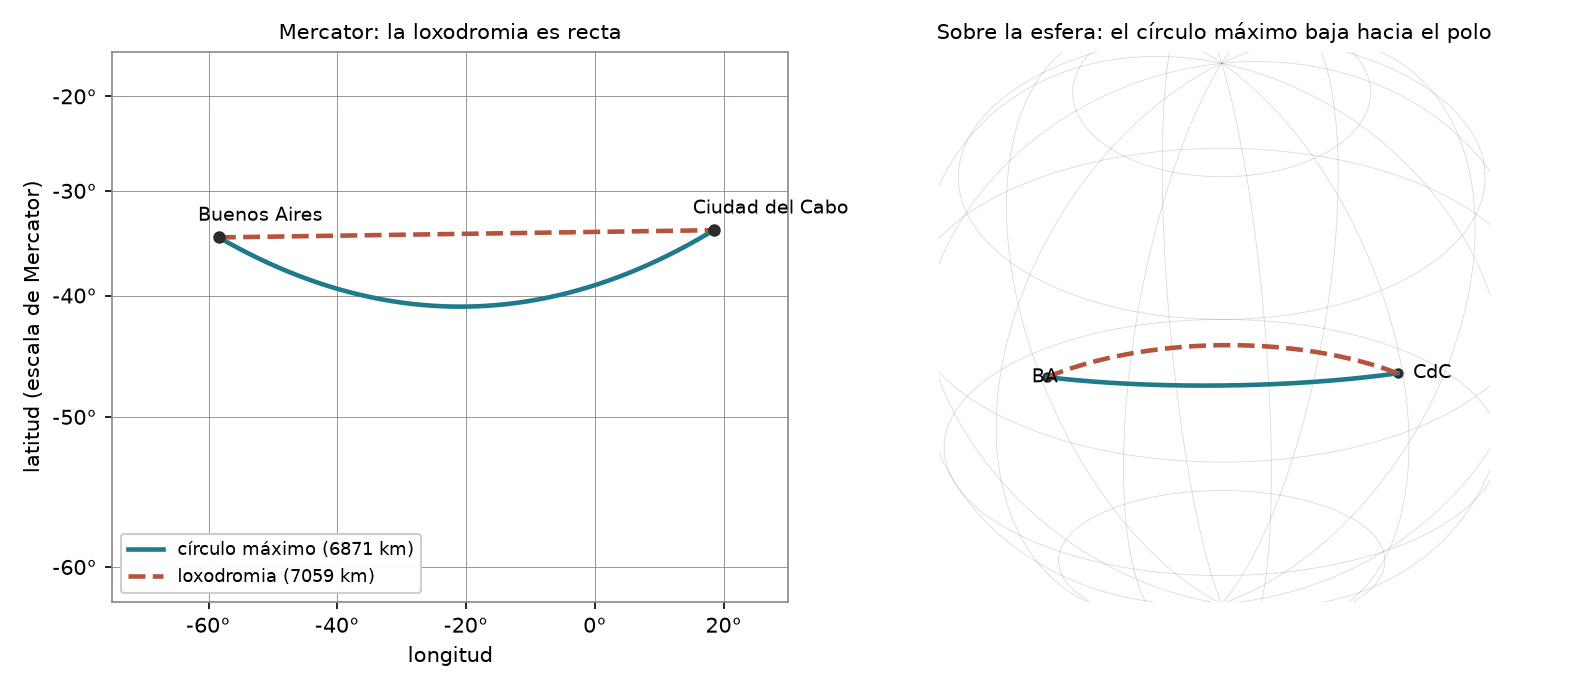
\includegraphics[width=\linewidth]{figuras/esfera/esfera_loxodromia.png}
\caption{Círculo máximo (teal) y loxodromia (rust, a trazos) entre Buenos Aires
\((-34{,}6^\circ;\ -58{,}4^\circ)\) y Ciudad del Cabo \((-33{,}9^\circ;\ 18{,}4^\circ)\),
coordenadas aproximadas, sobre la esfera de radio medio. A la izquierda, en la proyección de
Mercator; a la derecha, sobre la esfera. Generada con
\texttt{apunte/scripts/cap15\_trigonometria\_esferica.py}.}
\label{fig:esfera-loxodromia}
\end{figure}

\begin{ejemplo}[Buenos Aires -- Ciudad del Cabo]\label{ej:esfera-loxodromia}
Sobre la esfera de radio medio \(R_1=6\,371\,008{,}8\) m, el círculo máximo entre los dos
puntos de la figura~\ref{fig:esfera-loxodromia} mide \(6871\) km, parte con acimut
\(113{,}51^\circ\) y llega con acimut \(65{,}42^\circ\): el rumbo gira \(48{,}08^\circ\). Por
Clairaut, su latitud extrema es \(-40{,}99^\circ\), \(6{,}39^\circ\) al sur de Buenos Aires. La
loxodromia mantiene el rumbo \(89{,}37^\circ\) y mide \(7059\) km: \(189\) km más.
\end{ejemplo}

\subsection{Aplicación topográfica: de Buenos Aires a Mendoza, y el exceso de una red de control}

\paragraph{La esfera que reemplaza al elipsoide.} La Tierra se modela con un elipsoide
(capítulo~\ref{cap:elipsoide}), sobre el que no hay fórmulas cerradas para los problemas
directo e inverso. En una zona acotada se lo reemplaza por una esfera, y hay dos elecciones
habituales del radio: la \emph{esfera de Gauss} de radio \(\sqrt{MN}\), con \(M\) y \(N\) los
radios de curvatura del meridiano y del primer vertical en la latitud media
(sección~\ref{sec:radios-MN}), y la \emph{esfera de radio medio} \(R_1=(2a+b)/3\). Para GRS80
(\(a=6\,378\,137\) m, \(f=1/298{,}257222101\)), \(R_1=6\,371\,008{,}8\) m.

Como coordenadas aproximadas, declaradas como tales, tomamos Buenos Aires
\((-34{,}6^\circ;\ -58{,}4^\circ)\) y Mendoza \((-32{,}9^\circ;\ -68{,}8^\circ)\), y usamos
sus latitudes geodésicas como latitudes sobre la esfera. La latitud media es
\(-33{,}75^\circ\), donde \(M=6\,355\,126{,}3\) m, \(N=6\,384\,736{,}7\) m y
\(\sqrt{MN}=6\,369\,914{,}3\) m. El control es la geodésica sobre el elipsoide GRS80 que
calcula \texttt{pyproj.Geod(ellps='GRS80').inv}, con el algoritmo de Karney, de geographiclib. La
tolerancia declarada para cualquier esfera es la diferencia relativa máxima entre los radios
principales, \(e^2\approx6694\) ppm (en la latitud media, \((N-M)/M\approx4659\) ppm).

\emph{Problema inverso.} La fórmula del coseno da \(\sigma=8{,}808473^\circ\); los acimutes,
\(\alpha_1=278{,}1972^\circ\) en Buenos Aires y \(\alpha_2=283{,}9867^\circ\) al llegar a
Mendoza (contraacimut \(103{,}9867^\circ\)). El rumbo gira \(5{,}79^\circ\) en el camino: es la
convergencia de meridianos, y Clairaut lo controla, porque
\(\cos\varphi_1\sin\alpha_1=\cos\varphi_2\sin\alpha_2=-0{,}814727\).

\begin{center}
\begin{tabular}{lrr}
\toprule
Modelo & Distancia (m) & Diferencia con GRS80 \\
\midrule
Esfera de radio \(\sqrt{MN}\) & \(979\,290{,}6\) & \(-2109{,}5\) m \ (\(-2150\) ppm)\\
Esfera de radio \(R_1\) & \(979\,458{,}8\) & \(-1941{,}3\) m \ (\(-1978\) ppm)\\
Elipsoide GRS80 (control) & \(981\,400{,}1\) & --- \\
\bottomrule
\end{tabular}
\end{center}

Las dos esferas quedan dentro de la tolerancia declarada, pero a unos dos kilómetros del
elipsoide: para una línea de casi \(1000\) km, del orden de \(2\cdot10^{-3}\). La razón es la
dirección de la línea. Su acimut medio es de \(281{,}09^\circ\), casi oeste, y en esa dirección
el elipsoide se curva con el radio de la sección normal de Euler
(sección~\ref{sec:curvaturas-principales}),
\(R_\alpha=MN/(N\cos^2\alpha+M\sin^2\alpha)=6\,383\,635{,}9\) m, muy cerca de \(N\) y mayor
que \(\sqrt{MN}\), que es un promedio de todas las direcciones. El arco \(\sigma\) por ese
radio da una distancia a \(0{,}01\) m de la de GRS80; la coincidencia tan fina es en parte
fortuita (las latitudes geodésicas no son latitudes esféricas) y no es un método general,
pero muestra de dónde sale la diferencia. Los acimutes sobre la esfera difieren de los de la
geodésica de GRS80 (\(278{,}1469^\circ\) y \(283{,}9365^\circ\)) en \(181''\), unos tres
minutos: para orientar con precisión hace falta el elipsoide.

\emph{Verificación del problema directo.} Partiendo de Buenos Aires con
\(\alpha_1=278{,}1972^\circ\) y \(\sigma=8{,}808473^\circ\) (los valores completos del
inverso), las fórmulas del directo devuelven \(\varphi_2=-32{,}9000000000^\circ\),
\(\lambda_2=-68{,}8000000000^\circ\) y el mismo acimut de llegada: el error de cierre en
posición es de \(8\cdot10^{-9}\) m. La forma vectorial
\(\hat r_2=\cos\sigma\,\hat r_1+\sin\sigma\,t\) coincide con \(\hat r(-32{,}9^\circ;-68{,}8^\circ)\)
hasta \(10^{-15}\).

\emph{Contraste con la loxodromia.} La loxodromia de Buenos Aires a Mendoza tiene rumbo
constante \(281{,}1229^\circ\) y mide \(979\,706{,}6\) m sobre la esfera de radio \(\sqrt{MN}\):
\(416{,}1\) m más que el círculo máximo. Con rumbos cercanos al oeste y latitudes medias la
diferencia es chica en proporción (unos \(4\cdot10^{-4}\)), pero no nula.

\paragraph{El exceso en una red de control.} Consideramos un triángulo de una red de control
con vértices de coordenadas aproximadas, declaradas como tales: \(1=(-34{,}60^\circ;\
-58{,}40^\circ)\), \(2=(-34{,}90^\circ;\ -58{,}75^\circ)\) y \(3=(-34{,}42^\circ;\
-58{,}90^\circ)\). Las geodésicas de GRS80 miden \(46{,}202\) km (1--2), \(54{,}995\) km
(2--3) y \(50{,}068\) km (1--3). Usamos la esfera de Gauss en la latitud media
\(-34{,}64^\circ\), de radio \(\sqrt{MN}=6\,370\,531{,}5\) m; sobre ella los lados difieren de
los de GRS80 en \(+3{,}6\), \(+109{,}5\) y \(-77{,}0\) m, por el mismo efecto de dirección que
en Buenos Aires--Mendoza, lo que no afecta al exceso más allá de la milésima de segundo.

Los ángulos esféricos, por las normales, son
\[
  A_1=69^\circ\,46'\,06{,}99'',\qquad A_2=58^\circ\,20'\,48{,}39'',\qquad A_3=51^\circ\,53'\,10{,}13'',
\]
que suman \(180^\circ\,00'\,05{,}51''\): el exceso es \(\varepsilon=5{,}508''\). El área plana
por Herón es \(S=1083{,}69\) km\(^2\), con los lados esféricos o con los de GRS80, y
\(S/R^2=5{,}508''\): coincide con la suma de ángulos menos \(\pi\) hasta
\(4\cdot10^{-5}{}''\). La corrección de Legendre es \(\varepsilon/3=1{,}836''\) por ángulo, y
los ángulos corregidos,
\[
  69^\circ\,46'\,05{,}15'',\qquad 58^\circ\,20'\,46{,}55'',\qquad 51^\circ\,53'\,08{,}30'',
\]
coinciden con los del triángulo plano de los mismos lados con residuos menores que
\(2\cdot10^{-6}{}''\). Si la red se calculara en el plano sin esta corrección, cada triángulo
de este tamaño arrastraría \(5{,}5''\) de error de cierre angular que no proviene de las
mediciones: más que la precisión angular de una estación total de un segundo, y por lo tanto
algo que hay que separar antes de compensar.

\begin{resultado}[Receta para una red de control]
Calculá \(\varepsilon\approx S/R^2\) con el área plana del triángulo y \(R=\sqrt{MN}\) en la
latitud media; compará la suma de los ángulos medidos con \(180^\circ+\varepsilon\) (el
error de cierre es la diferencia); y resolvé el triángulo como plano con los ángulos
compensados menos \(\varepsilon/3\) cada uno.
\end{resultado}

\begin{idea}[Qué se conserva y qué no]
Al pasar de la esfera al elipsoide se pierde la invariancia por rotaciones, y con ella las
fórmulas cerradas; la esfera local sigue sirviendo para el exceso y para Legendre, pero no
para distancias y acimutes de precisión a cientos de kilómetros.
\end{idea}

\section{Ejercicios con solución}

\begin{ejercicio}\label{ex:esfera-lal}
En un triángulo esférico se conocen \(b=50^\circ\), \(c=70^\circ\) y el ángulo comprendido
\(A=80^\circ\). Hallá \(a\), \(B\), \(C\) y el exceso, y verificá el teorema del seno.
\end{ejercicio}
\solucion{Por el teorema del coseno,
\(\cos a=\cos50^\circ\cos70^\circ+\sin50^\circ\sin70^\circ\cos80^\circ=0{,}344846\), de modo
que \(a=69{,}8276^\circ\). Despejando del mismo teorema escrito en cada vértice,
\(\cos B=(\cos b-\cos a\cos c)/(\sin a\sin c)\) da \(B=53{,}4855^\circ\), y del mismo modo
\(C=80{,}3643^\circ\). Los tres cocientes \(\sin a/\sin A\), \(\sin b/\sin B\),
\(\sin c/\sin C\) valen \(0{,}953139\). El exceso es
\(80^\circ+53{,}4855^\circ+80{,}3643^\circ-180^\circ=33{,}8499^\circ\).}

\begin{ejercicio}\label{ex:esfera-polar}
Un triángulo esférico equilátero tiene sus tres ángulos de \(100^\circ\). Hallá el lado con
el teorema del coseno para los ángulos, el exceso y qué fracción de la esfera cubre. ¿Cuánto
miden lado y área sobre una esfera de \(6371\) km? ¿Por qué en el plano el problema no tiene
solución única?
\end{ejercicio}
\solucion{Con \(A=B=C\), el teorema~\ref{teo:coseno-angulos} da
\(\cos a=(\cos A+\cos^2A)/\sin^2A=\cos A/(1-\cos A)=-0{,}147956\), así que
\(a=98{,}5085^\circ\). El exceso es \(300^\circ-180^\circ=120^\circ=\tfrac23\pi\), y el área en
la esfera unitaria es \(\tfrac23\pi\), la fracción \(\tfrac{2\pi/3}{4\pi}=\tfrac16\) de la
esfera. Sobre \(R=6371\) km, el lado mide unos \(10\,954\) km y el área unos
\(85\,010\,745\) km\(^2\). En el plano los ángulos de un equilátero son siempre \(60^\circ\) y
no fijan el lado (todos los equiláteros son semejantes); en la esfera el radio da la escala.}

\begin{ejercicio}\label{ex:esfera-directo}
Desde el punto \((0^\circ;\ 0^\circ)\) del ecuador se parte con acimut \(45^\circ\) y se recorre
un cuarto de círculo máximo, \(\sigma=90^\circ\). Hallá el punto y el acimut de llegada con
las fórmulas del problema directo, comprobá el resultado con el inverso y verificá la
constante de Clairaut.
\end{ejercicio}
\solucion{\(\sin\varphi_2=\cos0^\circ\sin90^\circ\cos45^\circ=\tfrac{\sqrt2}2\), así que
\(\varphi_2=45^\circ\); \(\Delta\lambda=\operatorname{atan2}(\sin45^\circ,\ 0)=90^\circ\), así que
\(\lambda_2=90^\circ\). El acimut de llegada es
\(\operatorname{atan2}(\sin45^\circ,\ 0)=90^\circ\): se llega yendo hacia el este, en el punto
de latitud máxima del círculo. El inverso entre \((0^\circ;0^\circ)\) y \((45^\circ;90^\circ)\)
devuelve \(\sigma=90^\circ\), \(\alpha_1=45^\circ\) y \(\alpha_2=90^\circ\). Clairaut:
\(\cos0^\circ\sin45^\circ=\cos45^\circ\sin90^\circ=0{,}707107\).}

\begin{ejercicio}\label{ex:esfera-legendre}
Un triángulo de una red de control es equilátero, de \(40\) km de lado, sobre una esfera de
\(6371\) km. Estimá el exceso con \(S/R^2\), comparalo con el exacto de L'Huilier e indicá el
ángulo esférico y la corrección de Legendre.
\end{ejercicio}
\solucion{\(S=\tfrac{\sqrt3}4\cdot40^2=692{,}82\) km\(^2\) y
\(\varepsilon\approx S/R^2=1{,}7069\cdot10^{-5}\) rad \(=3{,}521''\). L'Huilier con
\(a=b=c=40/6371\) rad da también \(3{,}521''\). Cada ángulo esférico mide
\(60^\circ+\varepsilon/3=60{,}0003260^\circ\), o sea \(60^\circ\,00'\,01{,}174''\) (el
teorema del coseno para los lados, despejando \(\cos A\), da el mismo valor). La corrección de
Legendre resta \(1{,}174''\) a cada ángulo y devuelve los \(60^\circ\) del equilátero plano.}

\begin{ejercicio}\label{ex:esfera-paralelo}
Dos puntos están sobre el paralelo de \(-34{,}6^\circ\), separados \(10^\circ\) de longitud
(de \(-58{,}4^\circ\) a \(-68{,}4^\circ\)), en una esfera de \(6371\) km. Compará el largo del
arco de paralelo con el del círculo máximo e indicá los acimutes de partida y llegada del círculo
máximo y su latitud extrema. ¿Cuál de las dos curvas es una loxodromia?
\end{ejercicio}
\solucion{El arco de paralelo mide \(R\cos34{,}6^\circ\cdot10^\circ=915{,}29\) km; el círculo
máximo, \(914{,}91\) km: \(0{,}38\) km menos. El círculo máximo parte con acimut
\(267{,}1559^\circ\) (un poco al sur del oeste) y llega con \(272{,}8441^\circ\); por Clairaut
alcanza la latitud \(-34{,}7022^\circ\) a mitad de camino, más cerca del polo sur. El paralelo
corta a todos los meridianos con acimut \(270^\circ\): es la loxodromia de rumbo oeste, y no es
geodésica.}

\paragraph{Bibliografía del capítulo.}

\begin{itemize}
  \item \textbf{Hitchman}, \emph{Geometry with an introduction to cosmic topology}.
  \item \textbf{Rosenfeld}, \emph{Proyección Estereográfica}.
  \item \textbf{Mahecha}, \emph{Mecánica Clásica Avanzada}.
\end{itemize}
